%!TEX root = ../thesis.tex
%*******************************************************************************
%*********************************** First Chapter *****************************
%*******************************************************************************

\chapter{Hyperbolic Cone Surfaces}  %Title of the First Chapter
\section{Introduction}


\section{Hyperbolic Cone Surfaces and Geodesics}

\begin{defn} \label{ConeSurface}
	A \textit{hyperbolic cone-surface} $S$ is a surface that can be triangulated by finitely many hyperbolic geodesic triangles.
\end{defn}

\begin{exmp} \leavevmode
	\begin{enumerate}
		\item Any hyperbolic surface is a hyperbolic cone surface.
		\item Doubling of any hyperbolic geodesic polygon is a hyperbolic cone surface. It is clearly not a hyperbolic surface, since around vertices there are no neighbourbhoods isometric to hyperbolic disks.
	\end{enumerate}
\end{exmp}

\begin{defn} \label{ConePoint}
	A vertex in a triangle of the triangulation is contained in more than one triangle. The \textit{cone angle} of a vertex is the sum of all these vertex angles. A vertex whose cone angle is not equal to $2 \pi$ is called a \textit{cone point}. 
\end{defn}

\begin{exmp}\leavevmode
	\begin{enumerate}
		\item Hyperbolic surfaces do not have any cone points.
		\item When we double a polygon, we have conepoints at the vertices.
	\end{enumerate}
\end{exmp}

\noindent Note that if we remove cone points from $S$, we get an incomplete hyperbolic surface whose metric completion is $S$.

\begin{theorem}[Gauss-Bonnet Theorem] \label{thm:Gauss-Bonnet}
	Let $S$ be a cone surface(possibly with boundary) with $n$ conepoints of cone angles $\theta_1, \ldots, \theta_n$ then 
	\[\iint_{S} K dA + \int_{\partial S} \kappa_g ds + \sum_{i=1}^{n} \left(2\pi - \theta_i\right) = 2 \pi \chi(S)\]
	where $K$ denotes the Gaussian curvature, $\kappa_g$ denotes the geodesic curvature and $\chi$ is the Euler characteristic of $S$.
\end{theorem}

\begin{defn} \label{HyperbolicCone}
	Let $\theta \in (0, 2 \pi )$ and $h \in \mathbb{R}^{+}$. Define 
			$$\mathcal{S}_{h,\theta} = \{z \in \mathbb{D} ~ | ~ d_{\mathbb{H}}(0,z) < h \text{ and } 0 \leq \text{ arg}z \leq \theta\}.$$
	We define a hyperbolic cone $\mathscr{C}_{h,\theta}$ with cone angle $\theta$ and slant height $h$ to be the quotient of $\mathcal{S}_{h,\theta}$ obtained after gluing the geodesics $\text{arg}z=0$ and $\text{arg}z=\theta$ via the elliptic isometry $z \mapsto e^{i\theta}z$ fixing the origin.
\end{defn}

\subsection*{Local Picture at the cone point}

\noindent Given a conepoint $p$ with cone angle $\theta < 2 \pi$ on $S$, there are finitely many geodesic triangles $\{T_1^p, T_2^p, \ldots, T_n^p\}$ on $S$ such that:
\begin{enumerate}
	\item Every $T_i^p$ has $p$ as a vertex.
	\item $T_i^p$ is identified to $T_{i+1(\textup{mod } n)}^p$ via an edge containing $p$. Call this edge $e_{i+1(\textup{mod }n)}^p$ 
	\item Sum of the vertex angles of $T_i^p$'s at $p$ is $\theta$.
\end{enumerate}

\begin{figure}[h]
%		\labellist	
%	\small
%	\pinlabel $T_1^p$ at 755 470
%	\pinlabel $T_2^p$ at 650 590
%	\pinlabel $T_{n-1}^p$ at 200 500
%	\pinlabel $T_n^p$ at 210 340
%	
%	\pinlabel $\theta_1^p$ at 550 420
%	\pinlabel $\theta_2^p$ at 500 470
%	\pinlabel $\theta_{n-1}^p$ at 310 465
%	\pinlabel $\theta_n^p$ at 320 375
%	
%	\pinlabel $e_1^p$ at 650 370
%	\pinlabel $e_2^p$ at 650 460
%	\pinlabel $e_3^p$ at 570 590
%	\pinlabel $e_{n-1}^p$ at 340 530
%	\pinlabel $e_{n}^p$ at 290 430
%	\pinlabel $e_1^p$ at 330 310
%	\tiny
%	\pinlabel $S_{\frac{a_p}{4},\theta}$ at 400 450
%	\endlabellist

	\includegraphics[width=8cm]{Chapter1/conenbhd.pdf}
	\caption{$U_1^p$}
	\label{fig:conenbhd}
\end{figure}

Therefore, there are finitely many geodesic edges $\{e_1^p,\ldots,e_n^p\}$ such that:
\begin{enumerate}
	\item Every $e_i^p$ has $p$ as a vertex.
	\item $e_i^p$ and $e_{{i+1}(\text{mod } n)}^p$ are the edges of $T_i^p$
\end{enumerate}

\noindent Consider the subset $U_k^p$ of the Poincare disk constructed inductively as follows (See Figure~\ref{fig:conenbhd}):
\begin{enumerate}
	\item Fix $k \in \{1,2,\ldots,n\}$. Embed $T_k^p$ into the disk such that $p$ is at the origin.
	\item Embed $T_i^p$ into the disk such that the common edge of $T_i^p$ and $T_{i-1}^p$ containing $p$ is identified for $i = k, k+1(\textup{mod } n), \ldots, k+n-1(\textup{mod } n)$.
\end{enumerate}

Let $a_p$ be the infimum of all the distances from $p$ to vertices of $T_i^p$'s other than $p$ i.e., $a_p = \displaystyle \min_{i=1,\ldots, n} \textup{length}(e_i^p)$. $S_{\frac{a_p}{4}, \theta}$ is a subset of $U_k^p$ that does not contain any other vertex. Let $W$ be the subset of $S$ obtained after all edge identifications of $T_i^p$, therefore, $W$ is a quotient space of $U_k^p$. Restricting this quotient map to $S_{\frac{a_p}{4}, \theta}$, we get a quotient map onto the image of $S_{\frac{a_p}{4}, \theta}$ in $S$, which induces an isometric embedding of $\mathcal{C}_{\frac{a_p}{4}, \theta}$ into $S$ such that $0$ goes to $p$.

% https://q.uiver.app/?q=WzAsNSxbMCwxLCJTX3tcXGZyYWN7YV9wfXs0fSwgXFx0aGV0YX0iXSxbMSwxLCJXIl0sWzIsMSwiUyJdLFsxLDIsIlxcbWF0aGNhbHtDfV97XFxmcmFje2FfcH17NH0sIFxcdGhldGF9Il0sWzEsMCwiVV9rXnAiXSxbMCwzXSxbMywyLCIiLDIseyJzdHlsZSI6eyJ0YWlsIjp7Im5hbWUiOiJob29rIiwic2lkZSI6ImJvdHRvbSJ9fX1dLFswLDFdLFsxLDJdLFswLDQsIiIsMix7InN0eWxlIjp7InRhaWwiOnsibmFtZSI6Imhvb2siLCJzaWRlIjoidG9wIn19fV0sWzQsMV1d
\[\begin{tikzcd}
	& {U_k^p} \\
	{S_{\frac{a_p}{4}, \theta}} & W & S \\
	& {\mathcal{C}_{\frac{a_p}{4}, \theta}}
	\arrow[from=2-1, to=3-2]
	\arrow[hook', from=3-2, to=2-3]
	\arrow[from=2-1, to=2-2]
	\arrow[from=2-2, to=2-3]
	\arrow[hook, from=2-1, to=1-2]
	\arrow[from=1-2, to=2-2]
\end{tikzcd}\]


Note that $W = \bigcup_{i=1}^n T^p_i/ \sim$ is a quotient space of $U^p_k$. Moreover, under this quotient map $S_{\frac{a}{4}, \theta}$ goes to $\mathcal{C}_{\frac{a}{4}, \theta} \subset S$ . Therefore, $p$ has a neighbourhood in $S$ isometric to a hyperbolic cone. 

\begin{remark}\label{rem:disjoint_cone_nbhds}
	As there are only finitely many cone points, we can choose a $\delta > 0$ such that cone neighbourhoods of distinct cone points don't intersect. In \cite{PARLIER}, the authors prove that if cone angles are strictly less than $\pi$, then we can find cone neighbourhoods with slant heights depending only on cone angles. In other words, distinct cone points cannot be arbitrarily close if cone angles are strictly less than $\pi$.
\end{remark}

Let $\gamma$ be a piecewise simple regular curve passing through a conepoint $p$ and $\gamma_1, \gamma_2$ be the two arcs formed by $\gamma$, ending and starting at $p$ respectively. Assume $\gamma_1, \gamma_2$ lies in $T_i$ and $T_j$ respectively where $i < j$. Then, define
$$\Theta_1(\gamma) = \angle \gamma_1, e_{i+1} + \angle e_{i+1}, e_{i+2}+\cdots+\angle e_{j-1},e_{j} + \angle e_{j}, \gamma_2  $$
$$\Theta_2(\gamma) = \angle \gamma_2, e_{j+1} + \angle e_{j+1}, e_{j+2}+\cdots+\angle e_{i-1},e_{i} + \angle e_{i}, \gamma_1  $$

\begin{figure}[h]
	\includegraphics[width=8cm]{Chapter1/conenbhd2.pdf}
	\caption{$\Theta_1(\gamma)$ and $\Theta_2(\gamma)$}
	\label{fig:cone2}
\end{figure}

\noindent All these angles are calculated by lifting to $U_k^p$ for some $k$ and they are independent of $k$. Note that $\Theta_1(\gamma)+ \Theta_2(\gamma) = \theta < 2\pi$. This implies that atleast one of $\Theta_1(\gamma)$ and $\Theta_2(\gamma)$ is strictly less than $\pi$.    
%$$r_x = \sup_r \{B_r(x) \text{ is isometric to a hyperbolic disc}\}$$
%
%\noindent Note that when $p$ is a cone point, $h_p$ is the slant height of the largest embedded hyperbolic cone with vertex at $p$. 
%\begin{defn} \label{InjRadius}
%	The injectivity radius of a point $x \in S$, denoted by $\inj_x$, is defined as follows:
%	$$\inj_x = \max\{h_x, r_x\}$$
%	
%	The injectivity radius of a cone surface $S$ is defined as 
%	$$\inj(S) = \inf_x \inj_x $$
%\end{defn}
%
%\begin{prop} \label{InjRadiusPositive}
%	Let $S$ be a hyperbolic cone surface. Then, $\inj(S)   > 0$.
%\end{prop}
%\begin{proof}
%	Consider the compact subset $K \coloneqq S \setminus \bigcup_{p \in P} \mathscr{C}_{h_p} $ of $S$. Injectivity radius is continuous on $K$, since restricted to $K$ it is the usual injectivity radius. This implies that infimum is attained on $K$, say $i > 0$. Outside this compact set, every point has a injectivity radius bounded below by $\min_{p \in P} h_p$. Hence,   $\inj(S) = \min\{i,\bigcup_{p \in P} h_p\} > 0$.
%\end{proof}

\begin{defn} \label{Peripheral}
	A curve on $S$ is called \textit{conepoint peripheral} if it bounds a disk with cone points and if it bounds only one conepoint we call it just \textit{peripheral}.
\end{defn}

\begin{prop}\label{ShortCurves}
	There exists $M > 0$ such that any closed curve in $S \setminus P$ of length less than $M$ is either trivial or peripheral. 
\end{prop}

\begin{proof}
	Consider the compact subset $K$ of $S$ obtained after removing disjoint cone neighbourhoods around cone points. The existence of such disjoint cone neighbourhoods is given by Remark~\ref{rem:disjoint_cone_nbhds}. The injectivity radius is a continuous function on $S$, therefore, it will have an infimum on $K$, say $\frac{M}{2}$. Let $\gamma$ be closed curve in $S \setminus P$ of length less than $M$. Suppose $\gamma \cap K = \emptyset$, then it lies completely inside a cone neighbourhood, by connectedness of $\gamma$. This implies that it is either trivial or homotopic to a cone point. 
	Suppose $\gamma \cap K \neq \emptyset$, then there exists an embedded disk $B_{M/2}(x)$ around an $x \in \gamma \cap K$ such that $\gamma \subset B_{M/2}(x)$. This implies that $\gamma$ is trivial.
\end{proof}

%\begin{defn} \label{Angle}
%	Let $p$ be a conepoint. Let $\gamma$ be a curve passing through the cone point
%\end{defn}
\begin{defn}
	A \textit{geodesic} in a cone-manifold is a smooth curve which is locally length minimising.
\end{defn}
%\begin{prop} \label{prop:geodesic}
%	Let $S$ be a hyperbolic cone surface with cone angles  $< 2 \pi$. Then, a geodesic in $S$ cannot pass through cone points.
%\end{prop}
%\begin{proof}
%	Suppose a geodesic $\gamma$ passes through a cone point $p$. Let $\{T_1^p, \ldots, T_n^p\}$ be the geodesic triangles containing $p$ on $S$. Choose a small enough cone neighbourhood $C_p$ of $p$ such that $\gamma \cap C_p = \gamma \cap \left(C_p \cap \left(T_i \cup T_j\right)\right)$, for some $i<j$ i.e, the local picture looks like in the Figure \ref{fig:cone2}. Then, either $\Theta_1(\gamma)$ or $\Theta_2(\gamma)$ is less than $\pi$. Suppose $\Theta_1(\gamma) < \pi$, now lifting this to $U_i^p$, we see that, in no neighborhood of $p$ is $\gamma$ length-minimising. This is because we can shorten the curve by joining a point from the incoming arc to a point on the outgoing arc via a hyperbolic geodesic. Now, if $\Theta_2(\gamma) < \pi$, again lifting it to $U_j^p$, we see that $\gamma$ is not locally length-minimising.    
%\end{proof}

\begin{theorem} \cite[Theorem 5.1]{SPTAN} \label{thm:scgeodesic_existence}
Let $S$ be a hyperbolic cone surface with cone angles less than or equal to $\pi$. Let $\gamma$ be an essential simple closed curve in $S \setminus P$ i.e., non-peripheral and non-trivial simple closed curve. Then, there exists a unique simple closed geodesic representative $c$ in the free homotopy class of $\gamma$ in $S \setminus P$. 
\end{theorem} 

\begin{proof}
	Let $\mathscr{H}$ denote the free homotopy class of $\gamma$ in $S \setminus P$. As $\gamma$ is an essential simple closed curve, $l(\sigma) > M > 0$ for all $\sigma \in \mathscr{H}$, where $M$ is the value from Proposition~\ref{ShortCurves}. Hence, there exists $l > M$ such that $\inf_{\sigma \in \mathscr{H}} l(\sigma) = l $. 
	
	Now, let $\{\sigma_n\}_n$ be a sequence of curves such that $\{l(\sigma_n)\}$ is a decreasing sequence converging to $l$. Reparametrise these curves to be defined on the same interval with speed proportional to arc-length. We have an equicontinuous family of functions into the compact metric space $S$, thus, by Arzela-Ascoli, there exists a $c$ such that $\sigma_n \rightarrow c$ uniformly. 
	
	Suppose $c$ passes through a cone point $p$. Let $\mathcal{C}_p$ be the cone neighbourhood around the cone point $p$ and $U^p_n$ be a subset of Poincare disk as above such that $\mathcal{C}_p$ is a quotient of a subset of $U^p_n$. Now there are many choices for $U^p_n$ and we choose $n$ such that homotoping a curve off the origin doesn't change the free homotopy class in the surface. As $c$ passes through $p$, a conepoint of angle less than $\pi$, we could homotope $c$ off the point such that it decreases the length, thus contradicting minimality of $c$. This can be easily seen in $U_p^n \subset \mathbb{D}$. This implies that $c \subset S \setminus P$ and locally length-minimising, thus a geodesic.	
	
	For brevity, denote $S \setminus P$ by $\mathcal{S}$. Let $\widetilde{\mathcal{S}}$ be the universal cover of $\mathcal{S}$ identified with the Riemannian universal cover of $\mathcal{S}$ with complete hyperbolic metric, denote it by $\mathcal{S}^\prime$.
	
	\begin{figure}[h]
		\includegraphics[width=8cm]{Chapter1/simplicity.pdf}
		\caption{}
		\label{fig:simplicity}
	\end{figure}
	  
	Let $\tilde{c}$ be a lift of $c$ into $\widetilde{\mathcal{S}}$. Suppose $\tilde{c}$ has a transverse self-intersection, then there exists $x\in \widetilde{\mathcal{S}}$ such that two arcs of $\tilde{c}$ passes through $x$ with distinct tangents. Observe that $\text{dev}(\tilde{c})$ is a hyperbolic geodesic, since $\tilde{c}$ is a geodesic and $\text{dev}$ is a local isometry. This gives a contradiction, since at $\text{dev}(x)$, the geodesic $\text{dev}(\tilde{c})$ cannot have distinct tangents. Hence, $\tilde{c}$ is simple.
	
	 Let $c^\prime$ be the unique simple closed geodesic in the homotopy class of $\mathscr{H}$ in $\mathcal{S}^\prime$. As $c^\prime$ is simple, two distinct lifts of $c^\prime$ don't intersect in $\widetilde{\mathcal{S}}$ and they have distinct endpoints that are nested. Also, we know that the lifts $\tilde{c}^\prime$ and $\tilde{c}$ obtained by lifting the homotopy between $c^\prime$ and $c$ have the same endpoints at infinity. This implies that, distinct lifts of $c$ have distinct endpoints that are nested.
	
	As the endpoints are nested, two distinct lifts of $c$, if they intersect transversally must form a bigon, which implies that their developing images must form a bigon, which is impossible since they are hyperbolic geodesics. Hence, no two lifts of $c$ intersect.
	
	From above discussion, every lift of $c$ is simple and no two of its lifts intersect. Also, $c$ cannot be a multiple of any other closed curve, since it is a primitive element of the fundamental group. Hence, $c$ is simple.
	
	Suppose $c, d$ are two simple closed geodesic representatives of $\gamma$. Now, if $c, d$ intersect, then they form a bigon, which implies that the developing images of their lifts form a bigon. This is impossible because hyperbolic geodesics cannot form a bigon. Therefore, $c \cap d = \emptyset$. This implies that there is an embedded hyperbolic cylinder with $c$ and $d$ as its boundary circles. This is again a contradiction, since by Gauss-Bonnet there is no hyperbolic cylinder with two geodesic boundaries. This proves uniqueness. 
\end{proof}

The example below shows that the condition that cone angles less than $\pi$ is necessary. 

\begin{exmp}
	Take two copies of a right-angled hexagon and paste them as shown below in the Figure~\ref{fig:rtangledhex}. Then, we get a hyperbolic annulus with two cone points of cone angle $\pi$. Now, it is easy to see that the conepoint peripheral curve bounding these cone points has no simple closed geodesic representative in $S \setminus P$, since it degenerates to the geodesic joining the two conepoints.
	
	\begin{figure}[h]
		\includegraphics[width=7cm]{Chapter1/rtangledhex.pdf}
		\caption{}
		\label{fig:rtangledhex}
	\end{figure}
\end{exmp}

\begin{theorem}\label{thm:scgeodesic_existence2}
	Let $S$ be a hyperbolic cone surface with the set of cone points $P$ and all the cone angles are less than $2\pi$. Let $\gamma$ be an essential simple closed curve in $S$ such that $\gamma \subset S \setminus P$. There exists a geodesic $c$ freely homotopic to $\gamma$ in $S$ which does not pass through cone points.
\end{theorem}
\begin{proof}
	As $\gamma$ lies entirely within $S \setminus P$, it can be thought of as an essential simple closed curve in $S \setminus P$. By applying the usual Arzela-Ascoli argument as in \ref{thm:scgeodesic_existence}, we either get a geodesic representative or a curve $c$ passing through a cone point. In the latter case, we can homotope $c$, in $S$, off the cone point decreasing its length (since cone angles are less than $2 \pi$) but it would not be necessarily homotopic to $\gamma$ in $S \setminus P$.
	
	Now, repeating this process, we will either hit a geodesic representative or get an infinite sequence of curves of decreasing length. Now, by Arzela-Ascoli, we will get an infimum-realizing curve $\sigma$. And, $\sigma$ cannot pass through conepoints, because if it does, it would contradict the length minimality. 
\end{proof}

\section{Collars}\label{collars}

Let $S_{g,b,p}$ denote a surface of genus $g$ with $b$ boundary components and $p$ punctures/cone-points. From now on, we assume that our hyperbolic cone surfaces have cone-angles less than $\pi$ at every cone point.

\begin{defn}
	A hyperbolic annulus with geodesic boundaries and one cone-point i.e., $S_{0,2,1}$ is called a \textit{V-Piece}. A hyperbolic pair of pants i.e., $S_{0,3,0}$ is called a \textit{Y-piece}.
\end{defn}

\begin{defn} \label{partition}
	A partition of a cone-surface $S$ is a set of simple closed geodesics $\mathcal{P} = \{\gamma_1, \ldots, \gamma_n\}$ such that  $ S \setminus \mathcal{P}$ is a union of $Y$-Pieces and $V$-Pieces.
\end{defn}

\begin{lem} \label{partition:existence}
		Let $S$ be a hyperbolic cone surface with $n$ conepoints of cone angles less than $\pi$. Given any set $\mathcal{P}_1 = \{\gamma_1, \ldots, \gamma_k\}$ of disjoint, non-isotopic, non-conepoint peripheral essential simple closed geodesics of $S$, there exists a set $\mathcal{P}_2 = \{\gamma_{k+1}, \ldots, \gamma_m\}$ such that $\mathcal{P} = \mathcal{P}_1 \sqcup \mathcal{P}_2$ forms a partition for $S$ and $m = 3g-3+n$.
\end{lem}

\begin{proof}
	Let $S_1, \ldots, S_k$ be the connected components of $S \setminus \mathcal{P}_1$. Now, if any $S_i$ has genus greater than 1, then it has a non-peripheral simple closed geodesic. If any $S_i$ has genus 0, then it has to be $S_{0,b,n}, \textup{ where } b \geq 2$. Otherwise, it would imply that one of the $\gamma_i$'s is peripheral. 
	
	Therefore, any of these $S_i$ either:
	\begin{enumerate}
		\item contains a non-peripheral essential simple closed geodesic or
		\item is a $Y$-piece ($S_{0,3,0}$) 
		\item is a $V$-piece ($S_{0,2,1}$)
	\end{enumerate}
	
	Now, if $S_i$ contains a non-peripheral essential simple geodesic, repeat the above process until we end up with $Y$-pieces and $V$-pieces.
	
\end{proof}

\begin{lem}[Collar Lemma] \label{lem:collarlemma}
	Let $\mathcal{P} = \{\gamma_1, \ldots, \gamma_m\}$ be a partition of a hyperbolic cone surface $S$. Then, there exists pairwise disjoint neighbourhoods $\mathscr{C}_1, \ldots, \mathscr{C}_m$ of $\gamma_1, \ldots, \gamma_m$ respectively defined as:
		$$\mathscr{C}_i=\left\{z \in S ~\vert~ d(\gamma_i,z) \leq \textup{arcsinh}\left( \frac{\cos\left({\frac{\alpha}{2}}\right)}{ \sinh\left(\frac{l\left(\gamma_i\right)}{2}\right)}\right)\right\},\textup{for } i = 1,2, \ldots,m$$
	where $\alpha < \pi$ is the largest cone angle of $S$.
\end{lem}

\begin{proof}
	This is a special case of \cite[Theorem 3]{PARLIER}. As $P$ is a partition, $S \setminus P$ is a union of $Y$-Pieces and $V$-Pieces with boundary geodesics from $P$. Note that each geodesic from $P$ is part of atmost two of the pieces.
	
	Suppose $\gamma_k$ forms two boundary geodesics of a single $Y$-piece, then by Lemma~\ref{lem:collarlemmaY}, it follows that $\tilde{\mathscr{C}_k} = \left\{z \in S ~\vert~ d(\gamma_k,z) \leq \textup{arcsinh}\left( \frac{1}{ \sinh\left(\frac{l\left(\gamma_k\right)}{2}\right)}\right)\right\}$ 
	is a collar around $\gamma_k$ and $\mathscr{C}_k \subset \tilde{\mathscr{C}_k}$, since arcsinh is an increasing function.
	
	Suppose $\gamma_k$ forms boundary geodesics of two different $Y$-pieces, then by Lemma~\ref{lem:collarlemmaY}, it follows that $\tilde{\mathscr{C}_k} = \left\{z \in S ~\vert~ d(\gamma_k,z) \leq \textup{arcsinh}\left( \frac{1}{ \sinh\left(\frac{l\left(\gamma_k\right)}{2}\right)}\right)\right\}$ is a collar around $\gamma_k$ and $\mathscr{C}_k \subset \tilde{\mathscr{C}_k}$, since arcsinh is an increasing function.
	
	Similarly, using \ref{lem:collarlemmaV}, the cases when $\gamma_k$ forms the boundary geodesics of a single $V$-piece, two different $V$-pieces, and a $V$-piece and a $Y$-piece can be proved. 
	
\end{proof}
%
%\begin{cor}\label{collar}
%	Let $c$ be a non-peripheral, essential simple closed geodesic then there exists a neighbourhood of $c$ isometric to a hyperbolic cylinder. This neighbourhood is called a collar.
%\end{cor}
%
%\begin{proof}
%	This follows directly from Collar lemma, since given any non-peripheral simple closed geodesic, we can extend it into a partition.
%\end{proof}
\section{Simple Length Spectrum of hyperbolic cone surfaces}

Let $S$ be a surface with finitely many punctures. We start by proving two lemmas about filling curves.
\begin{defn}
	Let $a,b$ be distinct isotopy classes of closed curves. The intersection number of $a$ and $b$ denoted by $i(a,b)$ is defined as the infimum of the number of intersections over all representatives of $a$ and $b$ i.e.,
	$$i(a,b) = \inf_{\gamma \in a, \sigma \in b} |\gamma \cap \sigma|$$ 
\end{defn}
\begin{defn} \label{Filling}
		Let $\mathcal{F} = \{a_1, \ldots, a_n\}$ be a set of distinct isotopy classes of curves on $S$. Then, $\mathcal{F}$ is called a filling of $S$, if there exists curves $\tilde{\mathcal{F}} = \{\gamma_1, \ldots, \gamma_n\}$ in minimal position, where $\gamma_i$ is a representative for the class $a_i$, such that, $S \setminus \tilde{\mathcal{F}}$ is a disjoint union of disks or once-punctured disks. 
\end{defn} 

Let $\mathcal{F} =  \{a_1, \ldots, a_n\} $ be a filling of $\Sigma$ and $\gamma$ is a closed curve on $S$, then define
$$i(\gamma, \mathcal{F}) = \max_{i = 1,\ldots, n} i(\gamma, a_i) $$

\begin{lem} \label{lem:FillingLemma}
	Let $\mathcal{F}$ be a filling of $S$, possibly with boundary and punctures, consisting of non-peripheral essential simple closed curves. Define, for fixed $N \in \mathbb{N}$
	$$ \mathcal{I}_N = \{a ~ | ~ i(a,\mathcal{F}) \leq N, a \text{ is an isotopy class of a simple closed curve} \}. $$
	Then, $\mathcal{I}_N$ is a finite set for every $N \in \mathbb{N}$.
\end{lem}

\begin{proof}
	
	Give $S$ a complete hyperbolic structure and we denote the hyperbolic surface thus obtained also by $S$. If $S$ has cusps, then there are neigbourhoods around cusps such that every simple closed geodesic is disjoint from these neighbourhoods.

	Now, consider the geodesic representatives of curves in $\mathcal{F}$. Removing cusp neighbourhoods if any, we can assume that the surface is compact, possibly with non-geodesic boundary. 
	
	Now, $S \setminus \mathcal{F}$ is disjoint union of geodesic polygons or a geodesic polygons with an open disk removed. Let $a \in \mathcal{I}_N$, then the number of arcs corresponding to $a$ in each of these polygons is bounded above. This implies that the length of $a$ is also bounded above. We know that there are only finitely many simple closed curves with lengths bounded above by any given positive real number i.e., simple length spectrum of hyperbolic surface is discrete. Hence, $\mathcal{I}_N$ is a finite set. 
	
\end{proof}

\begin{defn}
	A filling $\mathcal{F}$ is said to be \textit{admissible} if it consists only of non conepoint-peripheral, essential simple closed geodesics.
\end{defn}

\begin{lem} \label{Admissible Filling:Existence}
	Every hyperbolic cone surface has an admissible filling.
\end{lem}

\begin{proof}
	Let $S$ be a hyperbolic cone surface and $\mathcal{P} = \{\gamma_1, \gamma_2, \ldots, \gamma_n\}$ be a partition of $S$. Then, $S \setminus \mathcal{P}$ is a union of $Y$-pieces and $V$-pieces. Any two boundary components of these pieces can be joined by a simple arc. In the case of a $Y$-piece, we get three disjoint simple arcs and for a $V$-piece we get one simple arc not passing through cone point. Now, we join these arcs in such a way that they form simple closed curves of $S$. Taking $\mathcal{P}$ along with the geodesic representatives of these newly constructed simple closed curves will give us an admissible filling. The simple closed geodesics formed this way would not be conepoint-peripheral because they non-trivially intersect atleast one of the $\gamma_i$ exactly once.
	
\end{proof}

\begin{defn} \label{def:sls}
	The set of lengths of simple closed geodesics on the cone surface away from cone points is said to be its \textit{simple length spectrum}.
\end{defn}

\begin{theorem}\label{thm:discrete_sls}
	The simple length spectrum of a hyperbolic cone surface $S$ with all cone angles less than $\pi$ is discrete.
\end{theorem}

\begin{proof}
	Denote by $\mathcal{C}_S$, the set of simple closed geodesics on $S$.
	Consider the following set $\mathcal{A}_L$ defined as
	$$\mathcal{A}_L \coloneqq \{c \in \mathcal{C}_S ~ |~ l(c) < L \}$$
	where $l(c)$ denotes the length of the geodesic $c$. Let $\mathcal{F} = \{a_1, \ldots, a_n\}$ be an admissible filling. Note that by Collar Lemma~(\ref{lem:collarlemma}), every curve in this filling has a collar around them. This implies that there exists $N \in \mathbb{N}$, such that for any geodesic with $l(c) < L$, the intersection with the filling, $i(c, \mathcal{F}) < N$. Thus, by Lemma~\ref{lem:FillingLemma}, the set $\mathcal{A}$ is finite, which gives us the theorem.	
\end{proof}

\begin{theorem}\label{discrete_sls_for_torus}
	The simple length spectrum of a hyperbolic torus $T$ with one cone point $p$ is discrete.
\end{theorem}

\begin{proof}

By Gauss-Bonnet theorem for cone surfaces (Theorem~\ref{thm:Gauss-Bonnet}), we see that the cone angle of a hyperbolic torus has to be less than $2 \pi$. Now, any isotopy class of a essential simple closed curve in the torus has a geodesic representative that does not pass through the cone point, by Theorem ~\ref{thm:scgeodesic_existence2}. As isotopy classes of essential simple closed curves in $T \setminus p$ is same as that of $T$, every isotopy class of essential simple closed curve in $T \setminus p$ has a geodesic representative. Now, using the same argument as above, we are done. 
\end{proof}

\begin{remark}
	By Section~\ref{sec:holonomy_of_hyp_surfaces}, it is easy to note that holonomy of a hyperbolic cone surface is non-elementary. Also, whenever we have an irrational cone angle, the holonomy representation is also indiscrete. Now, by Theorem~\ref{thm:closed_length_spectrum_is_dense}, we have that non-elementary indiscrete reprersentations have dense closed trace spectrum. By Theorem~\ref{thm:discrete_sls} and Theorem~\ref{prop:holonomy_of_geodesics}, we get that holonomy representation of cone surfaces have discrete simple trace spectrum. Thus, we have a family of examples of indiscrete non-elementary representations with discrete simple trace spectrum but dense closed trace spectrum.
\end{remark}
\section{Fenchel-Nielsen Coordinates for Hyperbolic Cone surfaces}\label{sec:FNCoordinates}

In this section, we parametrise the space of hyperbolic cone surfaces similar to the complete surfaces case. We exposit the results following \cite{PB}, \cite{HuipingPan}. 

%Let $\mathcal{HC}(g,\alpha_1,\ldots,\alpha_n)$ be the space of all hyperbolic cone metrics with $n$ conepoints of cone angles $\alpha_1, \ldots, \alpha_n$ considered upto isometries isotopic to the identity. 
%
%\begin{theorem}
% For $\alpha_i < \pi$, there exists $3(3g-3+n)$ simple closed curves such that their lengths determine a unique element in $\mathcal{HC}(g,\alpha_1,\ldots,\alpha_n)$.
%\end{theorem}
%
%From now on, we assume that the all the cone angles are less than $\pi$. For any given isotopy class of a non-peripheral simple closed curve $\gamma$, we define the \textit{length} of $\gamma$ to be the length of the unique geodesic in the isotopy class. Thus, for a fixed $\gamma$, 
%\[l^\gamma: \mathcal{HC}(g, \alpha_1, \ldots, \alpha_n) \rightarrow \mathbb{R}_{>0}\] 
%is the map which gives the length of $\gamma$ in the given hyperbolic cone surface.
\begin{defn}
	We call a graph $G$, a \textit{conic graph} of type $(g,n)$ if it satisfies the following:
	\begin{enumerate}
		\item It has $2g-2 +n$ vertices.
		\item It has $3g-3+n$ edges.
		\item Every vertex has degree either 2 or 3.
	\end{enumerate}
\end{defn}

\begin{prop}
	Any conic graph $G$ of type $(g,n)$ has $n$ vertices of degree 2 and $2g-2$ vertices of degree 3.
\end{prop}

\begin{proof}
	Let $V$ be the number of vertices in the graph $G$ and $v,w$ be the number of vertices of degree 2 and 3 repsectively. Then,
	\begin{align*}
		v + w = V &= 2g-2+n \\
		2v + 3w &= 2(3g-3+n) 
	\end{align*}
	Solving the above system of equations we get that, $v = n$ and $w = 2g-2$.
\end{proof}

%\begin{defn}
%	 Let $g,n \in \mathbb{N}$ such that $2g+n \geq 3$ and $\overline{\alpha}\coloneqq (\alpha_1, \ldots, \alpha_n) \in (0,\pi)^n$. A marked conic graph of type $(g,n,\overline{\alpha})$ is a conic graph of type $(g,n)$ with the following information:
%	 \begin{enumerate}
	%	 	\item $e_l \coloneqq (e_{ik},e_{jk^\prime})$.
	%	 	\item $a_m \coloneqq (e_{m1}, e_{m2}, \alpha_m)$ 
	%	 \end{enumerate}	 	
% 	Here, the tuples $e_l$ determine the edges and $a_m$ give weights to degree 2 vertices.
% 	We call a marked conic graph admissible if the above graph is connected
%\end{defn}

\begin{defn}
	Let $g,n \in \mathbb{N}$ such that $2g+n \geq 3$ and $\overline{\alpha}\coloneqq (\alpha_1, \ldots, \alpha_n) \in (0,\pi)^n$. Let $e_{ik}$ be symbols such that $i = 1,2, \ldots 2g-2+n$ and $k= 1,2$ or $k = 1,2,3$. Consider the following data:
	\begin{enumerate}
		\item $e_l \coloneqq (e_{ik},e_{jk^\prime})$.
		\item $a_m \coloneqq (e_{r1}, e_{r2}, \alpha_m)$ 
	\end{enumerate}
	In the first family of 2-tuples each symbol $e_{ik}$ occurs exactly once. Construct a graph with vertices $v_i = \{e_{i1},e_{i2},e_{i3}\}$ or $v_i=\{e_{i1},e_{i2}\}$ for $i = 1,2, \ldots, 2g-2+n$ and every tuple $e_l =(e_{ik}, e_{jk^\prime})$ above is an edge between $v_i$ and $v_j$. $a_m$ gives weight $\alpha_m$ to the vertices of degree 2. The graph thus constructed is called a \textit{marked cubic graph} of type $(g,n,\overline{\alpha})$, if it is a connected conic graph of type $(g,n)$.
\end{defn}

Given a marked conic graph $G$ of the type $(g,n,\overline{\alpha}), L \coloneqq (l_1,l_2,\ldots,l_{3g-3+n})\in \mathbb{R}^{3g-3+n}_+$ and $ T \coloneqq (\tau_1,\tau_2,\ldots,\tau_{3g-3+n}) \in \mathbb{R}^{3g-3+n}$, we construct a hyperbolic cone surface $S$ as follows:

For every vertex $v_i$ of degree two, we construct V-piece with boundary curves $\gamma_{i1},\gamma_{i2}$ and similarly, for every vertex $v_k$ of degree three, we construct Y-piece with boundary curves $\gamma_{k1},\gamma_{k2},\gamma_{k3}$ such that 
\begin{enumerate}
	\item $l_m$ gives the lengths of boundary curves corresponding to the tuple $e_m = (e_{ik},e_{jk^\prime})$ i.e., $\gamma_{ik},\gamma_{jk^\prime}$.
	\item $\alpha_m$ gives the cone-angle of the $V$-piece corresponding to the tuple $a_m =(e_{r1},e_{r2}, \alpha_m)$ i.e, the one with boundary curves $\gamma_{r1}, \gamma_{r2}$.   
\end{enumerate} 
Note that the above data completely determines the $V$ and $Y$ pieces upto isometry. 

Now, we glue these constructed pieces together using the last remaining tuple $T$. For every tuple $e_l = (e_{ik}, e_{jk^\prime})$, let $A_1$ and $A_2$ be the corresponding $V$ or $Y$ pieces with boundary curves $\gamma_{ik}, \gamma_{jk^\prime}$. We paste $A_1$ and $A_2$ along these curves as follows:
\[\gamma_{ik}(s)= \gamma_{jk^\prime}(\tau - s) \coloneqq \gamma_{k}(s)\]

Here, we assume that $\gamma_{ik}$ are parametrised on $S^1$. Proceeding as above, we get a hyperbolic cone surface, with $n$ conepoints with cone angles $\alpha_1, \ldots, \alpha_n$. Also, note that $(L,T)$ gives Fenchel-Nielsen type parameters for the constructed hyperbolic surface for a fixed conic graph $G$.

\begin{defn}
	Let $S_g$ be fixed topological surface of genus $g$ and $\{p_1, \ldots,p_n\} \subset S$. A \textit{marked hyperbolic cone surface} is given by the tuple $(X, \phi)$ where $ \phi: S \rightarrow X$ is a homeomorphism and $\phi(p_i)$ is a cone-point of $X$ for all $i$.
\end{defn}

Two marked hyperbolic cone surfaces $(X, \phi), (Y, \psi)$ are said to be equivalent if $\phi \circ \psi^{-1}$ is isotopic to an isometry. The space of all equivalence classes of such marked hyperbolic cone surfaces is denoted by $\mathcal{HC}(g, \alpha_1,\ldots,\alpha_n)$ where $\alpha_i$ is the cone angle at $p_i$.

The following theorem follows from \cite[Section 3]{HuipingPan}. This says that the construction stated above gives all the marked hyperbolic cone surfaces

\begin{theorem}\label{thm:FNCoordinates}
	Let $G$ be a marked conic graph of type $(g,n)$, where $g \geq 1, n \geq 1 \text{ or } g = 0, n \geq 6 $. There exists a bijective correspondence
	\begin{align*}
		\mathcal{HC}(g, \alpha_1,\ldots,\alpha_n) &\longleftrightarrow \mathbb{R}_+^{3g-3+n} \times \mathbb{R}^{3g-3+n} \\
		[(X, \phi)] &\mapsto (L,T)
	\end{align*}
	where $L, T$ are corresponding length and twist parameters with respect to $G$. 
	Moreover, the lengths of $12g-12+32n$ non-peripheral simple closed curves determines the marked hyperbolic cone surface.
\end{theorem}

\section{Holonomy of Hyperbolic cone surfaces} \label{sec:holonomy_of_hyp_surfaces}

Let $S$ be a hyperbolic cone surface and $P \subset S$ be the set of cone points in $S$. Then, note that $S \setminus P$ has a hyperbolic atlas. This gives us a developing map-holonomy pair, i.e., there exists a local isometry $\text{dev}: \widetilde{S\setminus P} \rightarrow \mathbb{H}^2$ and a homomorphism 
$\rho: \pi_1(S \setminus P) \rightarrow \pslr$ such that the following diagram commutes.

% https://q.uiver.app/?q=WzAsNCxbMCwwLCJcXHdpZGV0aWxkZXtTIFxcc2V0bWludXMgQ30iXSxbMiwwLCJcXG1hdGhiYntIfV4yIl0sWzAsMiwiXFx3aWRldGlsZGV7UyBcXHNldG1pbnVzIEN9Il0sWzIsMiwiXFxtYXRoYmJ7SH1eMiJdLFswLDEsIlxcdGV4dHtkZXZ9Il0sWzEsMywiXFxyaG8oZykiXSxbMCwyLCJnIiwyXSxbMiwzLCJcXHRleHR7ZGV2fSIsMl1d
\[\begin{tikzcd}
	{\widetilde{S \setminus P}} && {\mathbb{H}^2} \\
	\\
	{\widetilde{S \setminus P}} && {\mathbb{H}^2}
	\arrow["{\text{dev}}", from=1-1, to=1-3]
	\arrow["{\rho(g)}", from=1-3, to=3-3]
	\arrow["g"', from=1-1, to=3-1]
	\arrow["{\text{dev}}"', from=3-1, to=3-3]
\end{tikzcd}\]
The diagram gives us the following:
$$ \text{dev} \circ g = \rho(g) \circ \text{dev} $$

Also, the developing map is unique upto post-composing by an isometry of $\mathbb{H}^2$ i.e., if $\text{dev}_2: \widetilde{S\setminus P} \rightarrow \pslr$ is another developing map for $S$, then $\text{dev}_2 = A \circ \text{dev}_1$, where $A \in \pslr$. The corresponding holonomies differ by conjugation by an element of $\pslr$, i.e., $\rho_2 = A \cdot \rho_1 \cdot A^{-1}$. 

Given a hyperbolic cone surface, we can subdivide the triangulation on it such that interior of every triangle lies completely inside a chart in the hyperbolic atlas. Call this triangulation $\mathcal{T}$. Note that every cone point is a vertex in this triangulation. Fix a complete hyperbolic structure on $S \setminus P$ and identify $\widetilde{S \setminus P},  \pi_1(S \setminus P)$ with its universal cover and the corresponding deck transformations respectively. Lift the triangulation $\mathcal{T}$ to $\widetilde{S \setminus P}$. By our choice of triangulation, each of the lift of triangles map injectively into $\mathbb{H}^2$ under developing map. Note that some of the triangles have ideal vertices, which correspond to cone points on the surface. Now, we define a map $\text{dev}_{\#}$ from the set of vertices, say $\mathcal{V}$, of this triangulation into $\mathbb{H}^2$ induced by the developing map.

Let $\tilde{v} \in \mathcal{V}$ such that $\tilde{v} \notin \tilde{S \setminus P}$ i.e., $\tilde{v}$ is an ideal vertex. This corresponds to a conepoint $v$ in $S$. There exists a smooth geodesic $\gamma: [0,1] \rightarrow S$, such that $\gamma(1) = v$. Let $\widetilde{\gamma}: \left[0,1\right) \rightarrow \widetilde{S \setminus P}$ be the lift of $\gamma$. This implies that 
$\displaystyle \lim_{t \rightarrow 1^-} \tilde{\gamma}(t) = \tilde{v}$. Now, we define $\text{dev}_{\#}: \mathcal{V} \rightarrow \mathbb{H}^2$ as follows:
\begin{center}
	$\text{dev}_{\#}(\tilde{v})= 
	\begin{cases}
		\text{dev}(\tilde{v}), \text{ if } \tilde{v} \in \widetilde{S \setminus P} \\
		\displaystyle \lim_{t \rightarrow 1^-} \text{dev}(\tilde{\gamma}(t)), \text{ if } \tilde{v} \text{ is an ideal vertex.}
	\end{cases}$
\end{center}

\begin{prop}
	$\text{dev}_\#$ is well-defined.
\end{prop}

\begin{proof}
	It is clearly well-defined for vertices in $\widetilde{S \setminus P}$. Suppose that $\tilde{v}$ is an ideal vertex and $\tilde{\gamma}$ be a geodesic lift as above. As, dev is a local isometry, it preserves lengths of curves. Thus, it follows that $l(\text{dev}(\tilde{\gamma})) = 1$, since $l(\tilde{\gamma})=1$. Now, as $\text{dev}(\tilde{\gamma})$ is geodesic and $\mathbb{H}^2$ is complete, we get that the limit $\displaystyle \lim_{t \rightarrow 1^{-}} \text{dev}(\tilde{\gamma}(t))$ exists.
	
	Let $\tilde{\gamma}, \tilde{\sigma}$ are two different geodesics with the properties as above. In particular, they have the same endpoint at infinity. Now, again using that dev is a local isometry we prove that $\text{dev}_{\#}$ is independent of the choice of lift.
	\begin{align*}
	 d_{\mathbb{H}^2} \left(\text{dev}(\tilde{\gamma}(t)),\text{dev}(\tilde{\sigma}(t))\right)
		&\leq d(\tilde{\gamma}(t),\tilde{\sigma(t)}) \\
	\implies \displaystyle \lim_{t \rightarrow 1^{-}} d_{\mathbb{H}^2} \left(\text{dev}(\tilde{\gamma}(t)),\text{dev}(\tilde{\sigma}(t))\right) &\leq \displaystyle \lim_{t \rightarrow 1^{-}} d(\tilde{\gamma}(t),\tilde{\sigma(t)}) \\	\implies d_{\mathbb{H}^2} \left(\displaystyle \lim_{t \rightarrow 1^{-}}\text{dev}(\tilde{\gamma}(t)),\displaystyle \lim_{t \rightarrow 1^{-}}\text{dev}(\tilde{\sigma}(t))\right) &= 0
	\end{align*}
	
	Thus, $\text{dev}_{\#}$ is well-defined.
\end{proof}

We will use $\text{dev}_{\#}$ to prove a Ehresmann-Thurston principle for the holonomies of hyperbolic cone surfaces.

\begin{prop} \label{prop:holonomy_around_the _punctures}
	The holonomy around the punctures for hyperbolic cone surface $S$ is elliptic.
\end{prop}

\begin{proof}
	Let $\gamma$ be the peripheral simple closed curve around the puncture $p$. As we have identified $\pi_1(S \setminus P)$ as the deck transformations of the covering map corresponding to the complete hyperbolic structure,  $\gamma$ can be thought of as a parabolic isometry of $\mathbb{H}^2$. Let $\tilde{p} \in \partial \mathbb{H}^2$ be the fixed point of $\gamma$. We prove that $\text{dev}_{\#}(\tilde{p}) \in \mathbb{H}^2$ is a fixed point of $\rho(\gamma)$.
	\begin{align*}
			\rho(\gamma)(\text{dev}_{\#}(\tilde{p})) &= \rho(\gamma)(\lim_{t \rightarrow 1^-} \text{dev}(\tilde{\sigma}(t)) \\ 
			&= \lim_{t \rightarrow 1^{-}} \rho(\gamma) \text{dev}(\tilde{\sigma}(t))\\ 
			&= \lim_{t \rightarrow 1^{-}} \text{dev}(\gamma \cdot \tilde{\sigma}(t))\\ 
			&= \text{dev}_{\#}(\tilde{p}).
	\end{align*}

	
	The last equality follows because $\gamma \cdot \tilde{\sigma}$ is another smooth curve that ends at $\tilde{p}$. 
\end{proof}

\begin{theorem}\label{thm:holonomies_are_open}
	Let $\rho: \pi_1(S \setminus P) \rightarrow \pslr$ be the holonomy of a hyperbolic cone structure and let $\rho_n : \pi_1(S \setminus P) \rightarrow \pslr$ be a sequence of homomorphisms such that for any peripheral curve $\gamma$, $\rho_n(\gamma)$ is conjugate to $\rho(\gamma)$ and $\rho_n$ converges to $\rho$. Then, for large enough $N$, $\rho_n$ can be realised as the holonomy of a hyperbolic cone structure, for all $n \geq N$. 
\end{theorem}

\begin{proof}
	Let $d$ be the developing map corresponding to the holonomy $\rho$ i.e, $d : \widetilde{S \setminus P} \rightarrow \mathbb{H}^2$ is a $\rho$-equivariant local isometry. We will now construct maps $d_n: \widetilde{S \setminus P} \rightarrow \mathbb{H}^2$ such that they are $\rho_n$-equivariant and are developing maps of hyperbolic cone structure.
	
	Let $\widetilde{\mathcal{T}}$ be the lift of a triangulation as above and $\mathcal{\widetilde{V}}$ be its set of vertices. Now, let $\{v_1, \ldots, v_m\} \subset \mathcal{\widetilde{V}} $ be the minimal set of vertices such that every other vertex in $\widetilde{\mathcal{T}}$ is in the orbit of this set. We define a map $(d_n)_{\#}: \mathcal{\widetilde{V}} \rightarrow \mathbb{H}^2$ as follows:
	
	\begin{center}
		$(d_n)_{\#}(v)= 
		\begin{cases}
			d_{\#}(v), \text{ if } v \in \{v_1, \ldots, v_m\} \\
			\rho_n(\gamma) \cdot d_{\#}(v_i), \text{ if } v = \gamma \cdot v_i, \text{ for some } \gamma \in \pi_1(S \setminus P).
		\end{cases}$
	\end{center}
	
	Note that \[\displaystyle \lim_{n \rightarrow \infty} (d_n)_{\#}(v) = \displaystyle \lim_{n \rightarrow \infty} \rho_n(\gamma) \cdot d_{\#}(v_i) = \rho(\gamma) \cdot d_{\#}(v_i) = d_{\#}(v)\].
	
	Let $e$ be an edge with vertices $v, w$. Suppose $(d_n)_{\#}(v) = (d_n)_{\#}(w)$ for infinitely many $n$, then $d_{\#}(v) = d_{\#}(w)$ which is a contradiction since $v,w$ lie on a triangle and $d$ is injective on triangles in $\widetilde{\mathcal{T}}$. This implies that for large enough $n$, $(d_n)_{\#}(v) \neq (d_n)_{\#}(w)$. Passing to a suitable subsequence, define $d_n$ on $e$ such that it sends $e$ to the geodesic joining $(d_n)_{\#}(v)$ and $(d_n)_{\#}(w)$.
	
	Now, let $\Delta_1, \ldots, \Delta_m$ be the minimal set of triangles in $\widetilde{\mathcal{T}}$ such that every other triangle in $\widetilde{\mathcal{T}}$ can be obtained by a deck transformation on an element in this set. Take $\Delta_i$ homeomorphically to the geodesic triangle bounded by the images of its edges under $d_n$. Now, extend $d_n$ equivariantly to all of $\widetilde{S \setminus P}$.
	
	As $d_n$ are immersions, we can pull back the hyperbolic metric onto $\widetilde{S \setminus P}$. 
	
	% https://q.uiver.app/#q=WzAsNCxbMCwwLCJcXHdpZGV0aWxkZXtTIFxcc2V0bWludXMgUH0iXSxbMiwwLCJcXGxlZnQoXFxtYXRoYmJ7SH1eMixnX3tcXG1hdGhiYntIfV4yfVxccmlnaHQpIl0sWzAsMiwiXFx3aWRldGlsZGV7UyBcXHNldG1pbnVzIFB9Il0sWzIsMiwiXFxsZWZ0KFxcbWF0aGJie0h9XjIsZ197XFxtYXRoYmJ7SH1eMn1cXHJpZ2h0KSJdLFswLDEsImZfbiJdLFsyLDMsImZfbiIsMl0sWzAsMiwiXFxnYW1tYSIsMl0sWzEsMywiXFxyaG9fbihcXGdhbW1hKSJdXQ==
	\[\begin{tikzcd}
		{\widetilde{S \setminus P}} && {\left(\mathbb{H}^2,g_{\mathbb{H}^2}\right)} \\
		\\
		{\widetilde{S \setminus P}} && {\left(\mathbb{H}^2,g_{\mathbb{H}^2}\right)}
		\arrow["{d_n}", from=1-1, to=1-3]
		\arrow["{d_n}"', from=3-1, to=3-3]
		\arrow["\gamma"', from=1-1, to=3-1]
		\arrow["{\rho_n(\gamma)}", from=1-3, to=3-3]
	\end{tikzcd}\]
	From the above commutative diagram, we get that, given any deck transformation $\gamma$
	\begin{align*}
		(d_n \circ \gamma)^\ast (g_{\mathbb{H}^2}) &= (\rho_n(\gamma) \circ d_n)^\ast(g_{\mathbb{H}^2}) \\
		\implies \gamma^\ast \circ d_n^\ast (g_{\mathbb{H}^2}) &=d_n^\ast \circ \rho_n(\gamma)^\ast (g_{\mathbb{H}^2}) \\ 
		\implies \gamma^\ast(d_n^\ast(g_{\mathbb{H}^2})) &= d_n^\ast(g_{\mathbb{H}^2})
	\end{align*}
	
	As every deck transformation preserves the metric $d_n^\ast(g_{\mathbb{H}^2})$, the metric descends to $S \setminus P$ giving an incomplete hyperbolic metric.
	
	Thus, $(d_n, \rho_n)$ is developing-holonomy pair for an incomplete hyperbolic structure on $S \setminus P$ such that $\rho_n$ is elliptic around the peripheral simple closed curves. This implies that $\rho_n$ arises as holonomy of a hyperbolic cone structure.
\end{proof}

\begin{prop} \label{prop:holonomy_of_geodesics}
	Let $c$ be a simple closed geodesic in a hyperbolic cone surface $S$, which does not pass through cone points, then $\rho(c)$ is hyperbolic. Moreover, length of the geodesic $c$ is given by the translation length of $\rho(c)$.
\end{prop}

\begin{proof}
	Let $P$ be the set of cone points for $S$ and $\widetilde{S \setminus P}$ be the universal cover of $S \setminus P$. As $c$ is a geodesic in $S \setminus P$, it lifts to a geodesic $\tilde{c}$ in $\widetilde{S\setminus P}$. Now, thinking of $c$ as a deck transformation, $c \cdot \tilde{c}(t) = \tilde{c}(t+l(c))$, where $l(c)$ is the length of the geodesic $c$. Since dev is a local isometry, $\text{dev}(\tilde{c})$ is also a geodesic. We claim that $\text{dev}(\tilde{c})$ is fixed by $\rho(c)$. Observe that,
	\begin{align*}
		\rho(c)(\text{dev}(\tilde{c}(t))) = \text{dev}(c \cdot \tilde{c}(t))= \text{dev}(\tilde{c}(t + l(s)))
	\end{align*} 
	Hence, $\rho(c)$ is hyperbolic with axis $\text{dev}(\tilde{c})$ and translation length $l(c)$. 
\end{proof}

\begin{cor}
	There are infinitely many simple closed curves with hyperbolic image under the holonomy of a hyperbolic cone surface. 
\end{cor}

\begin{proof}
	This follows by Proposition~\ref{prop:holonomy_of_geodesics} and Theorem~\ref{thm:scgeodesic_existence2}.
\end{proof}

\begin{theorem}
	Given holonomy $\rho$ of any cone surface $S$ of genus $g\geq 1$ and $n$ cone points, there exists:
	\begin{enumerate}
		\item if $n>1$, a subsurface $F \subset S$ of genus $g$ and one boundary component such that $\rho|_F$ is discrete and faithful.
		\item if $n=1, g\neq 1$, a subsurface $F \subset S$ of genus $g-1$ and two boundary components such that $\rho|_F$ is discrete and faithful.
	\end{enumerate}	 
\end{theorem}

\section{Action of the Mapping Class Group on the relative character variety}

The set of all homomorphisms $\rho: \pi_1(S \setminus P) \rightarrow G$, for $G = \slr,$ or $\pslr$, denoted by  $\mathcal{R}_G(S \setminus P)$, is called a \textit{representation variety}. Given a representation from $\rho\in \mathcal{R}_{\pslr}(S \setminus P)$, it can be lifted to a representation in $\mathcal{R}_{\slr}(S \setminus P)$, since $\pi_1(S \setminus P)$ is a free group. We also see that $\mathcal{R}_{\pslr}(S \setminus P)$ is a quotient of $\mathcal{R}_{\slr}(S \setminus P)$ in the following way.
	\begin{align*}
\mathcal{R}_{\slr}(S \setminus P) &\longrightarrow \mathcal{R}_{\pslr}(S \setminus P) \\
	\rho &\longmapsto \pi \circ \rho
\end{align*}
where, $\pi: \slr \rightarrow \dfrac{\slr}{\{\pm I\}} \cong \pslr$ is the usual quotient map.

 The space of all representations with the image of peripheral curves having traces $t_i$, denoted by $\mathcal{R}_{\slr}(S,t_1,\ldots,t_n)$, is called a \textit{relative representation variety}. Note that relative representation varieties remain invariant under conjugation, since conjugation preserves traces. The quotient $\mathcal{R}_{\slr}(S,t_1,\ldots,t_n) / \slr$, under the conjugation action of $\slr$, is called a \textit{relative character variety}. It is denoted by $\mathcal{X}_{\slr}(S, t_1, \ldots, t_n)$. We define $\mathcal{X}_{\pslr}(S, |t_1|,\ldots,|t_n|)$ similarly. 
 
% Now, observe that,
% \[\mathcal{X}_{\pslr}(S, |t_1|,\ldots,|t_n|) = \bigsqcup_{\varepsilon_i = \pm 1 } \mathcal{X}_{\slr}(S, \varepsilon_1 t_1,\varepsilon_2 t_2,\ldots,\varepsilon_n t_n) \Big / \sim \]
% where $[\rho_1] \sim [\rho_2]$ if 


\begin{prop}\label{prop:HolMap}
	There is a natural 1-1 map from the Teichmuller space of hyperbolic cone surfaces with fixed cone-angles $(\alpha_1, \ldots, \alpha_n)$ to $\mathcal{X}_{\pslr}(S, |t_1|,\dots,|t_n|)$
	\[\text{Hol}: \mathcal{HC}(g,\alpha_1,\ldots,\alpha_n) \rightarrow \mathcal{X}_{\pslr}(S, |t_1|,\dots,|t_n|) \]
	where $t_i = 2\cos{\frac{\alpha_i}{2}}.$
\end{prop}

\begin{proof}
	Given any marked hyperbolic cone surface $[(X,\phi)]$, there exists a developing map $d: \widetilde{X \setminus \phi(P)} \rightarrow \mathbb{H}^2 $ where $\widetilde{X \setminus \phi(P)}$ is the Riemannian universal cover of $X \setminus \phi(P)$. This also gives a holonomy map $\rho: \pi_1(X \setminus \phi(P)) \rightarrow \pslr$, we can precompose this with $\phi_\ast$ to get $\rho \circ \phi_\ast: \pi_1(S \setminus P) \rightarrow \pslr$. Thus, we define $\text{Hol}\left([(X,\phi)]\right) = [\rho \circ \phi_\ast]$. This map is well-defined because the choice of developing map and marking would change the holonomy only upto conjugation.
	
	The map is one-one because a marked hyperbolic cone surface is determined by lengths of finitely many curves by Theorem~\ref{thm:FNCoordinates}. Thus, holonomy is determined by traces of finitely many curves. 
	
\end{proof}
\begin{remark} \label{rem:openness_of_holonomies}
	By Theorem~\ref{thm:holonomies_are_open}, we see that image of $\text{Hol}$ is an open subset of the relative character variety.
\end{remark}
In view of the above correspondence and Proposition~\ref{prop:holonomy_of_geodesics}, we can define a length function $l_\gamma: \mathcal{HC}(g,\alpha_1,\ldots,\alpha_n) \rightarrow \mathbb{R}^+ $ as follows:
\[l_\gamma(X) = 2 \cosh^{-1}\left(\frac{|\tra(\text{Hol}(X)(\gamma))|}{2}\right)\]
where $\gamma$ is a fixed non-peripheral simple closed curve. This implies that $l_\gamma$ is a continuous function, since trace is a continuous function. Also, $\text{MCG}(S)$ acts on the set of length functions as follows: 
\[\Phi \cdot l_\gamma (X) \coloneqq l_\gamma (\Phi \cdot X) = \l_{\Phi^{-1}(\gamma)} (X)\]
 
\begin{defn}
 	Let $S$ be a surface and $P = \{p_1,\ldots,p_n\}$ be a finite subset of $S$. The mapping class group of $S$ denoted as $\text{MCG}(S,P)$ is defined as the set of all homeomorphisms which fixes the set $P$ pointwise upto isotopy relative to the set $P$.
\end{defn}

Note that $\text{MCG}(S,P)$ acts on the $\mathcal{HC}(\alpha_1,\ldots, \alpha_n)$ as usual, i.e., $\Phi \cdot \left[(X,\phi)\right] = \left[ (X, \phi \circ \Phi^{-1}) \right]$. It is clearly well-defined.

\begin{theorem}\label{thm:mcg_action_is_prop_disc}
	$\text{MCG}(S,P)$ acts properly discontinuously on $\mathcal{HC}(g,\alpha_1,\ldots,\alpha_n)$.
\end{theorem}

\begin{proof}
	
	The proof follows exactly as in the case of closed surfaces.
	
	Let $K$ be a compact subset of $\mathcal{HC}(g,\alpha_1,\ldots,\alpha_n)$. Let $\gamma_1,\gamma_2$ be simple closed curves that fill $S$ i.e., $S \setminus (\gamma_1 \cup \gamma_2)$ is a disjoint union of finitely disks. Any $\Phi \in \text{MCG}(S,P)$ is completely determined by its action on $\gamma_1, \gamma_2$ and the permutation of the disks in $S \setminus (\gamma_1 \cup \gamma_2)$. 
	
	Now from the remark at the end of Section~\ref{sec:holonomy_of_hyp_surfaces}, the functions $l_{\gamma_1}, l_{\gamma_2}$ are bounded above and below on $K$. Suppose the action is not properly discontinuous, this means that there exists infinitely many $\Phi_n \in \text{MCG}(S,P)$ such that $(\Phi_n \cdot K) \cap K \neq \emptyset$. Moreover, there exists infinitely many distinct curves $\sigma_k \coloneqq \Phi_{n_k}^{-1}(\gamma_i)$ for $i = 1 \text{ or } 2$. Suppose not, then as $\Phi_{n}$ are determined by their action on $\gamma_i$ and by finiteness of disks in the complement of $\gamma_1 \cup \gamma_2$, we get a contradiction.
	
	We will now find a curve $\beta$ such that $\l_{\Phi_n^{-1}(\beta)} (X)$ is unbounded which contradicts the fact that $\l_\beta$ is bounded. Fix a partition $\mathcal{P}$ on $S$. Suppose there exists a $\beta \in \mathcal{P}$ such that $i(\beta, \sigma_k)$ is unbounded. Then, there exists $L > 0$ such that $l_\beta (X) < L$ for all $X \in K$ and in turn, by Lemma~\ref{lem:collarlemma}, this implies that there exists $w > 0$ such that \[l_{\sigma_k}(X) \geq w \cdot i(\beta, \sigma_k) \rightarrow \infty.\] 
	
	Now, the problem reduces to finding a partition $\mathcal{P}$ and $\beta \in \mathcal{P}$ such that $i(\sigma_k, \beta) \rightarrow \infty$. Suppose there exists a partition $\mathcal{Q}$ where this does not hold, i.e., $i(\beta_i,\sigma_k) < N$ for all $\beta_i \in \mathcal{Q} \text{ and } k$. This implies that the number of arcs of $\sigma_k$ in $S \setminus \mathcal{Q}$ is uniformly bounded. Thus, there exists an infinite subset of $\{\sigma_k\}$ such that they differ only by Dehn twists along $\mathcal{Q}$. There will be a further subset such that all of them are twisted along $\beta^\prime \in \mathcal{Q}$ atleast once. Now, choose the curve $\beta$ such that:
	\begin{enumerate}
		\item $i(\beta, \beta^\prime)=1$ and $\beta \cap \left(Q \setminus \{\beta^\prime\}\right) = \emptyset$, when $\beta^\prime$ is non-separating.
		\item $i(\beta, \beta^\prime)=2$ and $\beta \cap \left(Q \setminus \{\beta^\prime\}\right) = \emptyset$, when $\beta^\prime$ is separating.
	\end{enumerate}
\end{proof}

Let us denote the image of $\text{Hol}$ by $\mathcal{D}$. There is a natural action of $\text{MCG}(S,P)$ on $\chi(S,t_1,\ldots,t_n)$ that is given as follows:
\[\Phi \cdot [\rho] \coloneqq [\rho \circ \Phi_\ast^{-1}]\]
It is easy to see that the action is well-defined. Now, by Theorem~\ref{thm:mcg_action_is_prop_disc}, Proposition~\ref{prop:HolMap} and Remark~\ref{rem:openness_of_holonomies} we get invariant open subset $\mathcal{D}$ of relative character variety such that the action of $\text{MCG}(S,P)$ is properly discontinuous. Thus, $\mathcal{D}$ forms a domain of discontinuity for the $\text{MCG}(S,P)$ action on the relative character variety. 

\section{Simple Stability}

Let $F_n$ denote the free group on $n$ letters, i.e., $F_n = \langle a_1, \ldots, a_n \rangle$.We define the \textit{Cayley graph} of $F_n$, denoted by $\mathcal{C}(F_n)$ as follows: vertices of this graph is given by the elements of $F_n$ and two vertices $(w_1, w_2)$ have an edge between them if $w_1 w_2^{-1} \in \{a_1, \ldots,a_n,a_1^{-1},\ldots,a_n^{-1}\}$. Observe that $\mathcal{C}(F_n)$ is a regular $2n$-valence graph with countably many vertices. It can also be thought of as the universal cover of bouquet of $n$ circles, $B_n$, thus identifying the fundamental group of $B_n$ to $F_n$. 

\begin{figure}[h]
	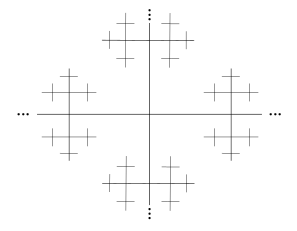
\includegraphics[width=8cm]{Chapter1/CayleyGraphF2.pdf}
	\caption{$\mathcal{C}(F_2)$}
	\label{fig:F2}
\end{figure}

Given a word $w \in F_n$, thinking of it as a loop $w: (S^1,1) \rightarrow (B_n, p)$, there exists a unique lift $\tilde{w}: \mathbb{R} \rightarrow \mathcal{C}(F_n)$ such that $\tilde{w}(0) = e$, where $e$ denotes the empty word. A word $w \in F_n$ is said to be \textit{primitive} if it belongs to some free generating set of $F_n$. 

Let $\rho: F_n \rightarrow \pslr$ be a representation and $p \in \mathbb{H}^2$ be a basepoint. We can define a map $\tau_{\rho,p}: \mathcal{C}(F_n) \rightarrow \mathbb{H}^2$ as follows:
\begin{itemize}
	\item $\tau_{\rho,p}(e) = p$.
	\item If $(v,w)$ is an edge in $\mathcal{C}(F_n)$, then it maps to the geodesic joining $\rho(v)(p)$ and $\rho(w)(p)$.
\end{itemize}
It is easy to note that $\tau_{\rho,p}$ as defined above is $\rho$-equivariant.

\begin{defn}
	A representation $\rho:F_n \rightarrow \pslr$ is said to be \textit{primitive-stable}, if there exists $C,\epsilon$ such that for any lift $\tilde{w}: \mathbb{R} \rightarrow \mathcal{C}(F_n)$ of a primitive word $w \in F_n$ the following holds for all $t,s \in \mathbb{R}$:
	\[\dfrac{1}{C}|t-s| - \epsilon \leq d(\gamma_{\tilde{w}}(t),\gamma_{\tilde{w}}(s)) \leq C|t-s|+ \epsilon\] 
	where $\gamma_{\tilde{w}} \coloneqq \tau_{\rho,p}(\tilde{w})$. Here, note that the constants $(C, \epsilon)$ are independent of the primtive word $w$ and its lift.
\end{defn}

\begin{exmp}
	\begin{enumerate}
		\item discrete and faithful representations by Svarc-Milnor Lemma.
		\item Schottky representations by \cite[Lemma 3.2]{Minsky}
	\end{enumerate}
\end{exmp}
\begin{prop}
	The holonomy representations are hyperbolic cone surfaces with more than one cone point and atleast one irrational cone angle are not primitive-stable.
\end{prop}

\begin{proof} 
	This follows from \cite[Lemma 3.2]{Minsky}. 
	
	Let $S_{g,n}$ be a surface with $n \geq 2$ punctures. Then, the fundamental group of $S_{g,n}$ is given by \[\pi_1(S_{g,n}) = \langle a_1, b_1,\ldots,a_g,b_g,c_1,\ldots,c_{n-1} \rangle\]
	where $a_i,b_i$ for handles and $c_k$ are homotopic to the punctures $p_k$. Let $X$ be hyperbolic cone surface structure on this surface with $n$ cone points and atleast one of them having an irrational cone angle. Without loss of generality assume that $p_1$ has an irrational cone angle, then $c_1$ will have an irrational elliptic image under the corresponding holonomy $\rho$. Also, note that all the $a_i, b_i$ have hyperbolic image. The subgroup generated by $\{a_1,c_1\}$ is a proper factor of $\pi_1(S_{g,n})$, but the image under $\rho$ i.e., $\langle \rho(a_1), \rho(c_1) \rangle$ is not Schottky, in fact it has dense image by \cite[Lemma 2.24]{MahanKoberdaKim}. Thus, $\rho$ is not primitive-stable.
\end{proof}

Note that for above proposition, the condition of more than one cone point is necessary because we know the holonomy of torus with one cone point is primitive-stable from \cite{LupiThesis}.

\begin{theorem}
	The holonomy representations of hyperbolic cone surfaces with rational cone-angles is primitive-stable.
\end{theorem}

\begin{proof}
	The holonomy representation of a hyperbolic cone surface with rational cone angles is discrete. Moreover, the image of the representation acts properly and cocompactly on the hyperbolic plane. Thus, the Cayley graph of $\pi_1(S \setminus P)$ is quasi-isometric to $\mathbb{H}^2$. This proves the statement. 
\end{proof}


Let $S$ be a hyperbolic cone surface with $n$ cone points $P \coloneqq \{p_1,\ldots,p_n\}$ and all cone angles less than $\pi$. 

\begin{defn}
	A representation $\rho:\pi_1(S \setminus P) \rightarrow \pslr$ is said to be \textit{simple-stable}, if there exists $C,\epsilon$ such that for any lift $\tilde{w}: \mathbb{R} \rightarrow \mathcal{C}(\pi_1(S \setminus P))$ of an essential simple closed curve $w \in \pi_1(S \setminus P)$, the following holds for all $t,s \in \mathbb{R}$:
	\[\dfrac{1}{C}|t-s| - \epsilon \leq d(\gamma_{\tilde{w}}(t),\gamma_{\tilde{w}}(s)) \leq C|t-s|+ \epsilon\] 
	where $\gamma_{\tilde{w}} \coloneqq \tau_{\rho,p}(\tilde{w})$. Here, again the constants $(C, \epsilon)$ are independent of the simple closed curve $w$ and its lift.
\end{defn}

\subsection*{Universal cover of $S \setminus P$}

Let $\widetilde{S \setminus P}$ be the universal cover of $S \setminus 	P$. Note that as $S$ is formed by pasting triangles, there exists a polygon $\mathcal{Q}$ such that $S$ is formed by side identifications of $\mathcal{Q}$ and all the cone points of $S$ form a subset of vertices of $\mathcal{Q}$ . Also, $\widetilde{S \setminus P} \coloneqq \mathcal{Q} \times \pi_1(S \setminus P) / \sim$. Let $d_{\widetilde{S \setminus P}}$ be the induced path metric on $\widetilde{S \setminus P}$. This is incomplete since we can have Cauchy sequences nearing to a ``lift of a cone point" but these sequences cannot converge as lifts of cone points are not in $\widetilde{S \setminus P}$.


We know that there exists a compact set $K \subset S$ such that $K \cap P \neq \emptyset$ and all the essential simple closed geodesics lie in $K$. This set $K$ is obtained by removing some cone neighbourhood around the cone points. Let $\widetilde{K}$ be the lift of $K$ under the Riemannian covering map.  

$d_{\tilde{K}}$ be the induced path metric on the subset $\tilde{K}$. It is easy to note that, for all $\tilde{x},\tilde{y} \in \tilde{K}$, \[d_{\widetilde{S \setminus P}}(\tilde{x},\tilde{y}) \leq d_{\tilde{K}}(\tilde{x},\tilde{y})\]

It is also important to note that $(\tilde{K}, d_{\widetilde{S \setminus P}})$ is locally isometric to $(\tilde{K},d_{\tilde{K}})$ i.e., for every $\tilde{x} \in \tilde{K}$, there exists a neighbourhood of $\tilde{x}$ in $(\tilde{K},d_{\widetilde{S \setminus P}})$ that is isometric to $(\tilde{K},d_{\tilde{K}})$. 

\begin{theorem}
	The holonomy representations of hyperbolic cone surfaces are simple-stable.
\end{theorem}

We will dedicate the rest of this section to prove the theorem:

\begin{lem}
	$\left(\tilde{K}, d_{\tilde{K}}\right)$ is a proper geodesic metric space.
\end{lem}
\begin{proof}
	We will prove that $\left(\tilde{K}, d_{\tilde{K}}\right)$ is length space which is complete and locally compact. This would give us the Lemma using \cite[Proposition 3.7]{BH}
	
	Given any $\tilde{x} \in \tilde{K}$, the image of $\tilde{x}$ under the covering map, say $x$, has a compact geodesic ball completely lying inside $K$. This will lift to a compact geodesic ball around $\tilde{x}$. This will also be a compact set in $(\tilde{K}, d_{\tilde{K}})$ since the geodesic ball lies completely in $K$. Hence, $\tilde{K}$ is locally compact.
	
	Let $(\tilde{x_n})$ be a Cauchy sequence in $(\tilde{K},d_{\tilde{K}}$. As $d_{\widetilde{S \setminus P}} \leq d_{\tilde{K}}$, $(\tilde{x_n})$ is also Cauchy in $(\tilde{K},\tilde{S \setminus P})$. Now, since $(\tilde{K},d_{\widetilde{S \setminus P}})$ is complete, there exists an $\tilde{x}$ such that $\tilde{x_n} \rightarrow \tilde{x}$. In other words, for any neighbourhood around $\tilde{x}$ in $(\tilde{K}, d_{\widetilde{S \setminus P}})$, all but finitely many $\tilde{x_n}$ lie in it. Now, there exists a geodesic neighbourhood in $(\tilde{K},d_{\tilde{K}})$ around $\tilde{x}$ isometric to a geodesic neighbourhood of $\tilde{x}$ in $(\tilde{K},d_{\widetilde{S \setminus P}})$. This implies that $\tilde{x_n}$ converges to $\tilde{x}$ in $(\tilde{K},d_{\tilde{K}})$.
	
	Hence, $(\tilde{K},d_{\tilde{K}})$ is a proper geodesic metric space.
	
	
\end{proof}
\begin{lem}
	$\mathcal{C}(\pi_1(S \setminus P))$ is quasi-isometric to $(\widetilde{K},d_{\tilde{K}})$.
\end{lem}

\begin{proof}
	The fundamental group $\pi_1(S \setminus P)$ acts as isometries on $\widetilde{S \setminus P}$ properly discontinuously. In particular, as $\tilde{K}$ is invariant under the action, $\pi_1(S \setminus P)$ acts properly discontinuously on $\tilde{K}$. Further, it acts cocompactly, as $K \cong \tilde{K}/\pi_1(S \setminus P)$. Now, by \v{S}varc-Milnor Lemma, the orbit map given by $\gamma \mapsto \gamma.\tilde{x}$ for any fixed $\tilde{x}$ is a quasi-isometry. 
\end{proof}

\begin{lem}
	There exists a geodesic 
\end{lem}
\begin{lem}
	Any subword of a cyclically reduced word representing a simple closed curve cannot contain $c_i^k$ as subword where $k > 1$.
\end{lem}
\begin{proof}
	This follows by Whitehead's lemma \cite[Corollary 4.3]{Minsky}
\end{proof}

\begin{lem}
	There exists a compact subset $K^\prime$ of $S \setminus P$ such that all ``subwords" of simple closed curves lie in $K^\prime$.
\end{lem}

\begin{lem}
	There exists a constant $C > 0$ such that for every subword $w$ of a simple closed curve in $S$,\[d_{\tilde{K}}(\tilde{x}, w \cdot \tilde{x}) \leq C \cdot d_{\widetilde{S \setminus P}}(\tilde{x}, w \cdot \tilde{x}).\]
\end{lem}
 
\begin{lem}
	The quasigeodesics in $\widetilde{S \setminus P}$ corresponding to 
\end{lem}



%********************************** %First Section  **************************************
